\chapter{Thermal History, Decoupling, and the Primordial Soup}

Last time the cosmological problem was organized geometrically: specify a scale-factor history \(A(t)\), specify the sign of the spatial curvature, and compare the resulting model with observation. In this lecture the emphasis shifts from geometry to thermodynamics. We want the temperature history of the universe. To do that carefully, we must first say what temperature means, how radiation acquires a thermal spectrum, why that spectrum survives after equilibrium is lost, and how a few rough but powerful estimates carry us backward from the \(3\,\mathrm{K}\) microwave background to recombination, radiation domination, and the primordial electron-positron soup. These notes follow Leonard Susskind's lecture closely; selected board frames preserved by LazyingArt LLC and Video2Book are kept where they stabilize visible equations and notation.

\section{From Expansion History to Thermal History}

The lecture opens with a short recap of the strategy from the previous chapter. One begins with a cosmological model, computes its consequences, and adjusts its parameters until it agrees with the data. For the present level of approximation the model is largely specified by two ingredients,
\begin{equation}
A(t),
\qquad
k = +1,0,-1,
\end{equation}
namely the scale-factor history and the sign of the spatial curvature.

From such a model one computes, at least in principle, two broad kinds of observables. One is the brightness of standard sources as a function of redshift. The other is the number of visible objects as a function of redshift. At moderate redshift these observations are more sensitive to the expansion history than to the curvature itself. That is why one can learn a good deal about \(A(t)\) before one knows \(k\) with much precision. The lecture briefly reminds us that the observational picture is consistent with a nearly flat universe and with an expansion history influenced by dark energy.

That recap is only a hinge. The real question now is different: what is the thermal history of the universe? Once we ask that question, the first issue is not yet cosmological. It is operational. What exactly do we mean by temperature?

\section{What Temperature Means: Equilibrium, Scattering, and the Box Model}

Susskind insists on a strict definition. Temperature is not merely a sensation of hot and cold. Temperature is a feature of thermal equilibrium. A system comes to thermal equilibrium through collisions and scattering, and it does so only if the microscopic equilibration time is short compared with the timescale on which the system itself changes. In cosmological language we may summarize the point schematically as
\begin{equation}
\tau_{\mathrm{scatt}} \ll \tau_{\mathrm{exp}}.
\end{equation}
When this inequality is true, the system has time to equilibrate before the background expansion significantly changes it.

To make the idea concrete, the lecture returns to the mythical box with perfectly reflecting walls. Suppose we fill the box with photons by shining in laser light and then close the hole. If there are only photons in the box, then almost nothing happens. The radiation bounces back and forth. Photons do not efficiently scatter from one another under ordinary conditions, so the pulse does not spread itself into a thermal distribution. A box containing only free radiation does not, by itself, thermalize.

Now put charged particles in the box. Electrons are especially efficient scatterers of electromagnetic radiation. An incoming electromagnetic wave shakes the charge; the accelerated charge re-radiates; scattering is strong. If the box contains a reasonable density of free electrons and protons, then the photons, electrons, and protons rapidly exchange energy and settle into a common thermal state.

The universe, however, is electrically neutral, so in the simplest model we take the particle content to be photons, electrons, and protons, with equal electron and proton densities,
\begin{equation}
n_{e^-} = n_p.
\end{equation}
If the electrons and protons are free, the radiation couples strongly to them. If instead they are bound into neutral hydrogen atoms, the situation changes drastically. Neutral atoms are poor scatterers. In the dilute present universe they are so poor at scattering that the photons do not come to equilibrium with matter on anything like the age of the universe. That is why the present universe is not in full thermal equilibrium.

\subsection{Question \& Answer}

\paragraph{Question.} If the microwave background has a temperature of about \(3\,\mathrm{K}\), why can we not simply say that the universe today has temperature \(3\,\mathrm{K}\)?

\paragraph{Answer.} Because the present universe is not a single equilibrated system. The microwave photons have a blackbody spectrum that can be characterized by a temperature, but the atoms, electrons, and other forms of matter are not in equilibrium with those photons. They do not share one common temperature. The modern universe therefore does not have one global thermodynamic temperature in the strict sense in which the lecture is using the word.

\section{Blackbody Radiation, Planck's Formula, and the Thermal Wavelength}

Once the box really is in thermal equilibrium, the next question is: what does the radiation look like? The box contains photons of many wavelengths or, equivalently, many frequencies, related by
\begin{equation}
\nu \lambda = c.
\end{equation}
The spectrum is described by an intensity function \(I(T,\nu)\), defined so that
\begin{equation}
dE = I(T,\nu)\, dV\, d\nu
\end{equation}
is the energy stored in a volume element \(dV\) within a frequency band \(d\nu\).

The lecture then follows a deliberate historical route. Before quantum theory, one had temperature, frequency, and the speed of light \(c\). Dimensional analysis then pushes one toward a Rayleigh--Jeans type law. Since Susskind debates the exact powers of \(c\) and the precise convention for intensity on the board, the safe lecture-faithful statement is the proportional one:
\begin{equation}
I_\nu^{\mathrm{classical}} \propto k_B T\, \nu^2.
\end{equation}
This has the correct low-frequency behavior, but as a complete formula it is disastrous. It grows without bound as \(\nu\) increases, so the integral over all frequencies would diverge. This is the ultraviolet catastrophe.

The remedy is to introduce a new constant, Planck's constant \(h\), and with it the blackbody formula:
\begin{equation}
I_\nu \propto \frac{h\nu^3}{e^{h\nu/(k_B T)}-1}.
\end{equation}
Again, the lecture's real use of this formula is not exact normalization but shape and scaling. The important thing is that the denominator contains the dimensionless ratio \(h\nu/(k_B T)\). For low frequency we can set
\[
x = \frac{h\nu}{k_B T},
\qquad
x \ll 1,
\]
so that \(e^x - 1 \approx x\). Then
\begin{align}
I_\nu
&\propto
\frac{h\nu^3}{e^{h\nu/(k_B T)}-1}
\approx
\frac{h\nu^3}{h\nu/(k_B T)}
=
k_B T\, \nu^2.
\end{align}
Thus the Planck spectrum reproduces the classical result in the low-frequency regime. The new physics appears when \(h\nu/(k_B T)\) is no longer small.

\begin{figure}[t]
\centering

\includegraphics[width=0.78\textwidth]{lecture_07_figure_02.png}
\caption{Thermal-wavelength inequality on the board. The upper line is partially clipped, but the crossover criterion is clear.}
\end{figure}

The board evidence captures the lecture's main point. The upper inequality is partially cut off but clearly indicates the threshold
\begin{equation}
\frac{h\nu}{kT} \gtrsim 1,
\end{equation}
and the lower line rewrites the same statement in wavelength form,
\begin{equation}
\frac{hc}{kT} \gtrsim \lambda.
\end{equation}
In the polished notation used in these notes, this becomes the characteristic thermal wavelength
\begin{equation}
\lambda_{\mathrm{th}} \sim \frac{hc}{k_B T}.
\end{equation}
This is not an exact replacement for Wien's numerical displacement law; it is the lecture's characteristic scale. The point is that once \(\lambda\) becomes shorter than \(hc/(k_B T)\), quantum suppression becomes strong, and the spectrum turns over rather than continuing to rise.

The lecture also extracts a scaling form from the Planck law. Ignoring overall constants that do not affect the shape, one may write schematically
\begin{equation}
I(\nu,T) \propto T^3 f\!\left(\frac{\nu}{T}\right).
\end{equation}
Therefore the shape of the blackbody curve depends only on the ratio \(\nu/T\). Changing the temperature mainly rescales the curve along the frequency axis.

\begin{figure}[t]
\centering
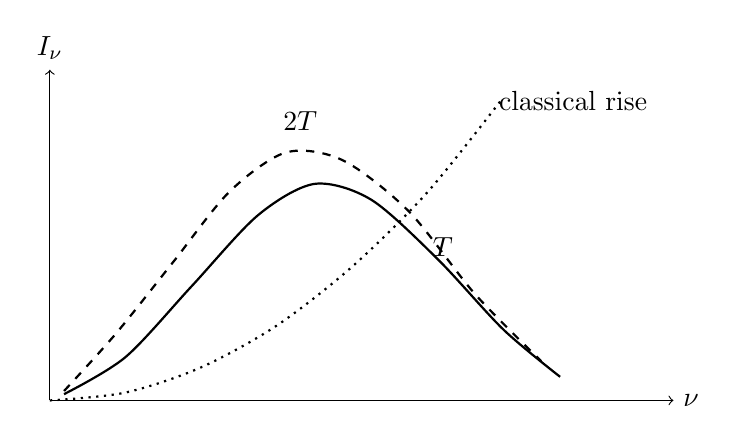
\begin{tikzpicture}[x=1.2cm,y=1.0cm]
\draw[->] (0,0) -- (6.6,0) node[right] {$\nu$};
\draw[->] (0,0) -- (0,4.2) node[above] {$I_\nu$};

\draw[dotted,thick] plot[smooth] coordinates
{(0.0,0.0) (0.8,0.10) (1.6,0.42) (2.4,0.95) (3.2,1.70) (4.0,2.65) (4.8,3.85)};

\draw[thick] plot[smooth] coordinates
{(0.15,0.08) (0.8,0.55) (1.5,1.45) (2.2,2.35) (2.8,2.75) (3.4,2.55) (4.1,1.80) (4.8,0.90) (5.4,0.30)};

\draw[dashed,thick] plot[smooth] coordinates
{(0.15,0.12) (0.7,0.85) (1.3,1.75) (1.9,2.65) (2.5,3.15) (3.1,3.05) (3.8,2.40) (4.5,1.35) (5.2,0.50)};

\draw (2.65,3.30) node[above] {$2T$};
\draw (3.95,1.95) node[right] {$T$};
\draw (4.65,3.80) node[right] {classical rise};
\end{tikzpicture}
\caption{Schematic blackbody spectra. The dotted curve indicates the classical continuation that leads to the ultraviolet catastrophe. The solid and dashed curves show the quantum turnover and the approximate rescaling of the spectrum when the temperature changes.}
\end{figure}

\subsection{Question \& Answer}

\paragraph{Question.} Why is the classical formula such a disaster, and what does the new constant \(h\) actually buy us?

\paragraph{Answer.} The classical formula keeps increasing with frequency, so it predicts an infinite total energy in the box. With only \(c\) available, there is no way to build a function that can turn the curve over. The introduction of \(h\) creates the dimensionless quantity \(h\nu/(k_B T)\). That quantity is small at low frequency, so the classical law is recovered, but it becomes large at high frequency, where the exponential suppression cuts off the spectrum. In the lecture's framing, that is the essential role of \(h\): it marks the boundary between the classical rise and the quantum fall.

\paragraph{Question.} Did Planck arrive at this formula from the same electron-proton box model used here?

\paragraph{Answer.} No. Susskind's point is historical as well as conceptual. Planck did not begin with the modern plasma picture. He used a combination of empirical curve fitting and what was already known from Wien's displacement law. What matters here is that the formula contains a new constant and that the new constant ties wavelength to temperature.

\section{Expansion, Decoupling, and the Frozen Blackbody Spectrum}

We now return from the box to the universe. Imagine that the box begins at sufficiently high temperature that electrons and protons are ionized. Then the charged particles scatter radiation efficiently, the whole system is in equilibrium, and the photon spectrum is blackbody.

Now expand the box. As it expands, the contents do work and cool. Eventually the temperature falls far enough that electrons and protons recombine into atoms. The scatterers disappear. The radiation then decouples from matter. After that point the system is no longer in full thermal equilibrium: atoms and radiation are free to go their separate ways.

And yet the lecture insists on a remarkable fact. The blackbody form of the radiation spectrum survives. The reason is simple and powerful. Expansion stretches every photon wavelength by the same factor. If the linear size of the box grows by a factor \(\alpha\), then
\begin{equation}
\lambda \mapsto \alpha \lambda,
\qquad
T \mapsto \frac{T}{\alpha}
\end{equation}
for the radiation spectrum. This is just the rescaling property already encoded in the dependence on \(\nu/T\). Thus one may summarize the cosmological rule as
\begin{equation}
\lambda \propto A,
\qquad
T \propto A^{-1}.
\end{equation}

This is why the microwave background today still has a blackbody spectrum, even though the universe today is far too cold and too dilute for radiation and matter to be in equilibrium. The spectrum is not blackbody because equilibrium is now being maintained. It is blackbody because that shape was frozen in when the universe was still ionized and has been carried forward by expansion ever since.

\subsection{Question \& Answer}

\paragraph{Question.} How can a blackbody spectrum remain blackbody after equilibrium has already been lost?

\paragraph{Answer.} Because the relevant feature is not the continued presence of scattering, but the uniform stretching of all photon wavelengths. Once the distribution has the blackbody shape, multiplying every wavelength by the same factor merely relabels the same shape by a lower temperature. That is exactly what the expansion of the universe does to free radiation after decoupling.

\section{Recombination Temperature from the Boltzmann Tail}

The next task is to estimate the temperature of recombination, or equivalently the temperature at which hydrogen would remain ionized. The naive argument is immediate: the ionization energy of hydrogen is
\begin{equation}
\epsilon_{\mathrm{ion}} \approx 13.6\,\mathrm{eV},
\end{equation}
so perhaps one should say that ionization persists until the characteristic photon energy is of order \(13.6\,\mathrm{eV}\), that is,
\begin{equation}
k_B T \sim \epsilon_{\mathrm{ion}}.
\end{equation}
But the lecture immediately warns that this is too naive.

\begin{figure}[t]
\centering

\includegraphics[width=0.72\textwidth]{lecture_07_figure_03.png}
\caption{Photon-energy notation and the photon-to-electron ratio on the board. The exponential is only partially written in the frame, but the lecture explicitly completes it as a Boltzmann factor.}
\end{figure}

The missing ingredient is abundance. There are vastly more background photons than electrons or protons:
\begin{equation}
\frac{N_\gamma}{N_e} \sim 10^8.
\end{equation}
So the right question is not whether the average photon has ionizing energy. The right question is whether the high-energy tail contains enough ionizing photons per atom. Susskind introduces the notation \(\epsilon\) for photon energy and writes the Boltzmann weight
\begin{equation}
P(\epsilon) \propto e^{-\epsilon/(k_B T)}.
\end{equation}
Evaluated at the ionization energy, this gives the fraction of photons energetic enough to ionize hydrogen. Multiplying by the photon-to-electron ratio, the criterion for roughly one ionizing photon per atom is
\begin{equation}
10^8 e^{-\epsilon_{\mathrm{ion}}/(k_B T)} \sim 1.
\end{equation}
This is the lecture's crucial estimate. Taking logarithms,
\begin{align}
\frac{\epsilon_{\mathrm{ion}}}{k_B T}
&\sim \ln 10^8
\approx 20,
\\[4pt]
k_B T
&\sim
\frac{\epsilon_{\mathrm{ion}}}{20}.
\end{align}
So the recombination temperature is not of order the full ionization energy. It is lower by a factor of order \(20\), and Susskind then remarks that a more careful treatment may push the factor closer to \(40\). The estimate is intentionally rough, but the physical point is sharp: because there are so many photons, the tail matters.

In the lecture's running estimate this places decoupling at about
\begin{equation}
T_{\mathrm{dec}} \sim 4\times 10^3\,\mathrm{K},
\end{equation}
with the clear caveat that the exact numerical factor is not the point.

\subsection{Question \& Answer}

\paragraph{Question.} Why does recombination happen at a temperature much lower than the hydrogen ionization energy?

\paragraph{Answer.} Because the average photon is not the correct standard. There are about \(10^8\) photons per electron. Even when the typical photon energy is far below \(13.6\,\mathrm{eV}\), the exponentially small tail of the distribution still contains enough photons above threshold to keep hydrogen ionized. Recombination therefore waits until the tail itself has become too sparse, not until the average photon energy has fallen below threshold.

\subsection{Question \& Answer}

\paragraph{Question.} If recombination emits \(13.6\,\mathrm{eV}\) photons, why does that not leave a dramatic spectral line in the final microwave background?

\paragraph{Answer.} Because as long as the evolution is slow enough, the system remains very close to thermal equilibrium while recombination is happening. Emission, absorption, and scattering keep redistributing the radiation so that the spectrum relaxes back toward the thermal form. Only if the expansion were fast enough to force a more abrupt freeze-out would one expect a pronounced bump to survive.

The lecture also answers a natural side question here. The enormous ratio \(N_\gamma/N_e \sim 10^8\) is taken to be essentially frozen in all the way back to decoupling, because between decoupling and the much hotter pair-production epochs there is no important mechanism for changing the total number of CMB photons or the total number of electrons and protons.

\section{Scale Factor, Last Scattering, and the Limit of Electromagnetic Observation}

Now the same estimate becomes geometrical. The characteristic wavelength of the microwave background today is the expanded remnant of the characteristic wavelength at decoupling, so
\begin{equation}
\frac{\lambda_0}{\lambda_{\mathrm{dec}}}
=
\frac{A_0}{A_{\mathrm{dec}}}
=
\frac{T_{\mathrm{dec}}}{T_0}.
\end{equation}
Here \(T_0\) means specifically the temperature of the microwave background today, not the temperature in a laboratory, not the kinetic temperature of gas in interstellar space, and not any averaged temperature of present matter. With
\[
T_0 \approx 3\,\mathrm{K},
\qquad
T_{\mathrm{dec}} \sim 4\times 10^3\,\mathrm{K},
\]
we get
\begin{equation}
\frac{A_0}{A_{\mathrm{dec}}}
\sim
\frac{4\times 10^3\,\mathrm{K}}{3\,\mathrm{K}}
\sim 10^3.
\end{equation}
Thus the universe has expanded by about a factor of a thousand since it became transparent.

This is the lecture's first clean thermal landmark. Before decoupling the universe was ionized and therefore opaque to electromagnetic radiation. Photons scattered too strongly from the charged plasma to travel freely across cosmic distances. After decoupling the universe became transparent, and the radiation we now call the CMB began to stream essentially freely toward us.

The observational picture is therefore shell-like. Looking farther away in space means looking farther back in time. Optical and other electromagnetic astronomy carries us backward until we arrive at the surface of last scattering. Beyond that the universe was opaque, so ordinary electromagnetic observation stops there.

The lecture returns, near its end, to an easy confusion. The CMB is indeed older than galaxies. But the fact that we see the CMB back to decoupling tells us nothing directly about whether there are galaxies today beyond the region from which their light can reach us. It tells us only how far electromagnetic radiation can carry direct information backward. What supports the usual extrapolation is something else: the observed homogeneity of galaxies as far out as we can see, with no visible sharp edge.

\subsection{Question \& Answer}

\paragraph{Question.} Does decoupling mark the end of all possible observation, or only the end of ordinary electromagnetic observation?

\paragraph{Answer.} Only the latter. The lecture's claim is that electromagnetic radiation cannot directly show us epochs earlier than decoupling, because the pre-decoupling universe was opaque to light. But particles that interact more weakly, such as neutrinos, could in principle escape from earlier times. Gravitational radiation would be even less impeded. So decoupling marks the observational wall for light, not necessarily the final wall for every conceivable messenger.

\section{Earlier Landmarks: Equality, Pair Creation, and the Asymmetry Puzzle}

Having reached decoupling, the lecture keeps going backward. The next landmark is the crossover between matter domination and radiation domination. Matter and radiation scale differently with the expansion:
\begin{equation}
\rho_m \propto A^{-3},
\qquad
\rho_r \propto A^{-4}.
\end{equation}
Therefore the ratio scales as
\begin{equation}
\frac{\rho_m}{\rho_r} \propto A.
\end{equation}

To estimate the present ratio, Susskind uses a deliberately crude but illuminating counting argument. There are about \(10^8\) photons per proton. Each CMB photon has characteristic energy of order \(10^{-4}\,\mathrm{eV}\), while a proton carries energy of order \(10^9\,\mathrm{eV}\). So, using only ordinary matter at first,
\begin{equation}
\left(\frac{\rho_m}{\rho_r}\right)_0
\sim
\frac{10^9\,\mathrm{eV}}{10^8 \times 10^{-4}\,\mathrm{eV}}
\sim 10^5.
\end{equation}
Then the lecture corrects itself: dark matter was omitted. Including dark matter multiplies the matter density by roughly a factor of ten, so the rough ratio becomes
\begin{equation}
\left(\frac{\rho_m}{\rho_r}\right)_0 \sim 10^6.
\end{equation}
Since \(\rho_m/\rho_r \propto A\), equality occurred when the scale factor was smaller than today by the same factor,
\begin{equation}
\frac{A_{\mathrm{eq}}}{A_0} \sim 10^{-6},
\qquad
\frac{T_{\mathrm{eq}}}{T_0} \sim 10^6.
\end{equation}
So going backward beyond decoupling, one reaches an even earlier epoch in which radiation, not matter, controlled the energy budget and therefore the expansion law.

\subsection{Question \& Answer}

\paragraph{Question.} Why does the lecture keep emphasizing ratios of \(A\) rather than absolute values of \(A\)?

\paragraph{Answer.} Because in a nearly flat universe the absolute normalization of the scale factor is not directly meaningful. A flat space does not have a finite radius of curvature whose size \(A\) could literally measure. What is meaningful is the expansion factor between two times. Thus \(A_0/A_{\mathrm{dec}}\), \(A_0/A_{\mathrm{eq}}\), and similar ratios carry physical information, while an isolated value of \(A\) does not.

Going back still farther, the temperature reaches about
\begin{equation}
T \sim 10^{10}\,\mathrm{K},
\qquad
\frac{A_0}{A} \sim 10^{14},
\end{equation}
so that the characteristic photon energy is of order
\begin{equation}
\epsilon_\gamma \sim 1\,\mathrm{MeV}.
\end{equation}
Now photon collisions can create electron-positron pairs:
\begin{equation}
\gamma\gamma \leftrightarrow e^- e^+.
\end{equation}
At this point the abundance of electrons and positrons is no longer controlled by what survives to the present. It is controlled by equilibrium at the current temperature. That is what Susskind means when he says that the number is no longer determined by ``memory of the future.''

In this hot plasma the electrons, positrons, and photons are all present in roughly comparable abundance, up to a tiny excess. The sum \(N_{e^-}+N_{e^+}\) can change because pair creation and annihilation change it continuously. But the difference does not change:
\begin{equation}
N_{e^-}-N_{e^+}=\mathrm{constant}.
\end{equation}
In the intermediate regime described in the lecture, before proton-antiproton pair creation becomes important, this conserved excess is essentially the proton number required by electrical neutrality.

Now comes the final inversion of the lecture. Since the total number of electrons plus positrons in the hot soup is of the same order as the photon number, while the surviving excess is only of order the present electron number, one infers
\begin{equation}
\frac{N_{e^-}-N_{e^+}}{N_{e^-}+N_{e^+}} \sim 10^{-8}.
\end{equation}
That means that in the primordial electron-positron soup there was roughly one excess electron for every \(10^8\) electron-positron pairs.

This turns the old puzzle upside down. One might have asked: why are there so many photons? The lecture's answer is that the sharper question is the opposite one: why is the excess of matter over antimatter so tiny? Why is
\[
N_{e^-}-N_{e^+}
\]
so small compared with
\[
N_{e^-}+N_{e^+}?
\]
The lecture stops there on purpose. The microscopic theory of that asymmetry is postponed to the next chapter.

There is one further observational remark near the end. Across the visible universe the sign of the excess appears to be the same. We do not see antigalaxies sending us antinuclei; we see the ordinary sign everywhere we can test it. The lecture regards a local statistical fluctuation of this size over the observed volume as wildly implausible. At the same time, it also stresses intellectual restraint: beyond the horizon we do not directly know what there is.

\section{Summary}

The lecture begins with geometry and turns to thermodynamics. Temperature is defined through equilibrium, equilibrium through scattering, and the box model teaches us immediately why free charges matter and neutral atoms do not. Once the box is in equilibrium, radiation is described by a blackbody spectrum, and the key dimensionless ratio \(h\nu/(k_B T)\) tells us where the classical description fails and quantum suppression takes over.

From there the lecture becomes cosmological. Expansion stretches wavelengths, so a blackbody spectrum can survive long after matter and radiation fall out of equilibrium. The present CMB is therefore understood as a frozen thermal relic. Using the huge ratio \(N_\gamma/N_e \sim 10^8\) together with the Boltzmann tail, one finds that recombination occurs not at the full ionization temperature of hydrogen but at a much lower temperature, of order \(4\times 10^3\,\mathrm{K}\). This in turn implies that the universe has expanded by about a factor of \(10^3\) since decoupling.

Going backward still farther, one reaches matter-radiation equality, then the electron-positron pair-production era, where equilibrium fixes particle abundances directly. The final result is not a completed theory but a sharpened mystery: the primordial soup was almost symmetric, with only one excess electron for roughly every \(10^8\) electron-positron pairs. That tiny excess, not the mere abundance of photons, is the real puzzle carried forward to the next lecture.